% !TEX program = xelatex
\documentclass[11pt, a4paper]{ctexart}

\usepackage[margin=2.6cm]{geometry}
\usepackage{booktabs}
\usepackage{graphicx}
\usepackage{amsmath}
\usepackage{array}
\usepackage{caption}
\usepackage[hidelinks]{hyperref}

\captionsetup{font=small, labelfont=bf}
\title{从缓存计量到来源证据：AI 内容审计中的上下文复用判定}
\author{殷一天\\
{\small 新疆大学，乌鲁木齐}}
\date{2026 年 9 月}
% TODO(作者确认)：投稿前补充邮箱；署名与单位按新疆大学口径暂填，请核对。

\begin{document}
\sloppy
\maketitle

\begin{abstract}
在 AI 内容治理中，判断“是否由模型生成”之外，更需要回答“内容从哪里来、是否同源”。本文提出并实证一条独立于文件与文本的证据通道：大模型 API 为计费而输出的上下文缓存计量。我们把审计者设定为合法持有计量记录、不持有他人正文的一方，将其任务形式化为“判定两次生成是否复用同一上下文”，并给出最简判定规则（缓存命中 token 数 $> 0$ 即判定复用）。在真实平台上执行两组受控调用：（1）裸 API 通道 8 次调用中，凡与锚点共享文档前缀的调用命中稳定为 512 token（占输入的 73.6\%--74.4\%），异文档与跨模型层级调用命中为 0，判定正确率 7/7，且该信号在约 35 分钟后仍可观测；（2）agent 编排通道 17 次受控调用\textbf{全部零命中}，机制分析定位到根因——编排框架把每次运行唯一的产物路径写入系统提示，请求前缀在第 172 个字符处分叉，缓存匹配从结构上不可能。研究表明：计量信号本身强而稳定，但其可用性取决于调用链路设计；结合《人工智能生成合成内容标识办法》的核验与日志留存要求，该通道可作为隐式标识的独立旁证，同时存在“未命中不等于不同源”（跨模型层级）与复用行为可观测的双刃边界，需在最小必要原则下使用。

\noindent\textbf{关键词：} 人工智能内容治理；来源审计；上下文缓存；计量取证；生成合成内容标识
\end{abstract}

\section{引言}

生成式人工智能进入大规模应用阶段后，内容治理的焦点正在从“是否为机器生成”转向“内容从哪里来、经由谁传播、风险落在何处”。这一转向有其技术与制度双重背景。技术一侧，通用检测器的可靠性边界已被反复论证：Sadasivan 等展示了改写攻击下检测准确率可以退化到随机猜测水平\cite{sadasivan2025tmlr}，把“判别真伪”作为唯一治理抓手并不稳固。制度一侧，我国《人工智能生成合成内容标识办法》自 2025 年 9 月 1 日施行，明确要求生成合成内容携带显式标识与元数据隐式标识，传播平台承担核验义务，服务提供者留存日志不少于六个月\cite{cac2025labeling}。制度设计已经预置了“标识—核验—留存”的证据链，但一个关键问题仍然悬空：\textbf{当标识在传播中被剥离、篡改或缺失时，是否还存在独立于文件本身的证据通道，能够回答“两批内容是否同源”？}

本文注意到一条被忽视的线索。为降低成本与延迟，主流大模型 API 普遍启用服务端上下文缓存，并把缓存使用情况写进计费响应：命中的输入 token 数与未命中的输入 token 数被分开计量\cite{deepseekcache}。这是一份\textbf{平台自己出具、随每次调用自动产生的确定性记录}。与文本水印相比，它不依赖内容载体的完整性；与文件元数据相比，它不随文件搬运而丢失；与时序侧信道相比\cite{song2025earlybird,wu2025iknow}，它不需要攻击者式的精细测量——记录里直接写着答案。自然的问题是：这份记录能不能用作来源审计的证据？

本文将这一问题形式化并给出首批实证。我们把审计者设定为\textbf{合法持有计量记录、不持有他人正文}的一方（平台合规、监管核验、权利人取证），把审计目标设定为“判定两次生成是否复用了同一段上下文”。通过在真实平台上执行两组受控调用——一组经由 agent 编排链路，一组为裸 API 调用——我们得到一个具有操作意义的双层结论：计量信号\textbf{本身是强信号}，在裸 API 通道上同源与异源完全可分；但它的可用性\textbf{高度依赖调用链路的设计}，在典型的 agent 编排链路中该信号会因系统提示注入运行时唯一路径而被结构性抹除。本文的主要贡献如下：

\begin{itemize}
\item \textbf{提出计量取证路径并量化其分离度（C1）}：以计费字段中的缓存命中计量为唯一信号，给出最简判定规则；在受控实验中同源复用稳定呈现 512 token 命中，异源为 0，形成完全分离。
\item \textbf{揭示并解释通道依赖性（C2）}：同一平台、同一账号、同一文本，经由 agent 编排链路的 17 次受控调用\textbf{全部零命中}；通过解析编排框架自身的请求日志，定位到根因——系统提示中嵌入了每次运行唯一的产物目录路径，使请求前缀在首百 token 内即分叉。审计可用性因此是链路设计的函数，而非平台能力的函数。
\item \textbf{给出制度衔接与边界分析（C3）}：计量取证可充当隐式标识的独立旁证，且现行留存义务使记录天然可得；但受“跨模型缓存命名空间”限制（同一文档跨层级调用命中为零），且信号同时构成对复用行为的可观测面，需要在最小必要原则下使用。
\end{itemize}

\section{相关工作}
\label{sec:related}

与本文相关的文献可以归入三条线索。

\subsection{AI 生成内容检测与来源归因}
围绕“机器生成文本能否被可靠识别”，已有研究给出了较强的否定性结论：Sadasivan 等系统地考察了检测器在改写攻击下的失效边界，指出通用检测难以作为可靠的长期防线\cite{sadasivan2025tmlr}。与之相对，水印与内容凭证走的是一条“主动嵌入可验证信号”的路线：Kirchenbauer 等提出基于词表划分的统计水印，在解码阶段嵌入可检验的信号\cite{kirchenbauer2023watermark}；工业界则推动内容凭证（Content Credentials）等元数据方案，把来源信息写入文件。两条路线的共同前提是信号必须随内容一起传播——一旦内容被替换载体、重新排版或跨平台搬运，文件层信号的可核验性就依赖平台执行核验义务。

\subsection{推理侧缓存的隐私副作用}
近两年，推理服务的性能优化暴露出一类新的信息泄漏面。Song 等发现共享 KV 缓存与语义缓存会引入时序侧信道，攻击者借助计时测量与分类模型判定缓存命中，进而逐 token 恢复他人的系统提示与提示前缀（TIFS）\cite{song2025earlybird}。Wu 等进一步揭示了多租户场景下 KV 缓存共享导致的提示泄漏路径\cite{wu2025iknow}。这类工作确立了“缓存状态可以被外部观测”这一事实，但其视角是\textbf{攻击者推断他人内容}；信号载体是细粒度计时，目标是最小化可观测窗口。

\subsection{前缀缓存系统}
Prompt Cache 等工作把“复用请求间重叠前缀的注意力状态”系统化为可模块化的推理加速技术，显著降低首 token 延迟与单位成本\cite{gim2024promptcache}。主流 API 平台已将磁盘级上下文缓存作为默认能力开放，并\textbf{在计费响应中显式给出命中计量}。本文关注的正是这一显式计量的“副作用”：它把缓存复用从隐蔽的时序现象变成了账面上的确定性字段。

\subsection{本文与已有工作的区别}
\begin{table}[t]
\centering
\small
\caption{本文与最近工作的定位对比}
\label{tab:position}
\begin{tabular}{p{2.6cm} p{4.2cm} p{4.6cm}}
\toprule
 & 缓存侧信道攻击\cite{song2025earlybird,wu2025iknow} & 本文 \\
\midrule
角色 & 恶意租户（攻击者） & 授权审计者（平台 / 监管 / 权利人） \\
信号 & 计时测量 + 分类器推断 & 平台计费字段（官方计量） \\
目标 & 窃取他人提示/系统提示 & 判定两次生成是否复用同一来源上下文 \\
场景 & 在线、多租户、实时 & 事后、单账号或平台侧、取证 \\
信号可得性 & 需精细实验设计 & 记录中直接可得（但依赖调用通道） \\
\bottomrule
\end{tabular}
\end{table}

\section{背景、审计模型与政策依据}
\label{sec:background}

\subsection{磁盘上下文缓存的命中规则}
DeepSeek API 的上下文缓存默认开启，官方文档给出了三条持久化规则\cite{deepseekcache}：（1）\textbf{请求边界持久化}：每次请求在用户输入结束处与模型输出结束处各产生一个缓存前缀单元；（2）\textbf{共同前缀检测}：当系统检测到多个请求存在共同前缀时，把该前缀持久化为独立单元；（3）\textbf{固定区间切分}：对长输入/输出按固定 token 区间切分单元。后续请求只有与某个缓存前缀单元\textbf{完全匹配}才会命中；官方同时说明命中“尽力而为”，缓存“数小时到数天”内自动清除。响应中给出两个计量字段：\texttt{prompt\_cache\_hit\_tokens} 与 \texttt{prompt\_cache\_miss\_tokens}。

\subsection{审计者模型}
本文把“审计者”定义为\textbf{合法持有计量记录、但不持有他人正文}的一方，例如：平台合规团队、依《人工智能生成合成内容标识办法》第九条必须留存日志的服务提供者、或在自身账号范围内取证的权利人。审计者可见：账单与 usage 记录（输入/输出 token 数、缓存命中/未命中数、时间戳、模型标识）；不可见：请求正文与他人生成结果。在此约束下，审计问题被表述为：\textbf{给定两次生成的计量记录，判断二者是否复用了同一段上下文}（同一文档、同一模板、同一底稿）。

\subsection{政策依据}
我国《人工智能生成合成内容标识办法》\cite{cac2025labeling}自 2025 年 9 月 1 日起施行：第五条要求在文件元数据中加入隐式标识（生成合成属性、服务提供者名称或编码、内容编号）；第六条要求传播平台\textbf{核验}元数据隐式标识，无法核验到但检测到显式标识或其他生成合成痕迹的，标记为疑似；第九条要求服务提供者对未加显式标识的导出内容\textbf{留存日志不少于六个月}；第十条禁止恶意删除、篡改、伪造、隐匿标识。该办法确立了“标识 + 核验 + 留存”的治理框架，但对“标识被剥离后如何独立核验来源关系”未给出技术手段——这正是计量取证可以补位的位置。

\section{方法：计量取证与受控实验设计}
\label{sec:method}

\subsection{判定规则}
设审计者观察到的第 $i$ 次生成记录为
$u_i = (c_i, m_i, o_i)$，其中 $c_i$、$m_i$ 分别为缓存命中与未命中的输入 token 数，$o_i$ 为输出 token 数。本文的最小判定规则为
\begin{equation}
\mathrm{reuse}(u_j \mid u_i) =
\begin{cases}
\text{是}, & c_j > \tau \\
\text{否}, & c_j \le \tau
\end{cases}
\qquad (\tau = 0),
\label{eq:rule}
\end{equation}
即：只要后续请求出现非零缓存命中，就判定其复用了先前出现过的上下文。规则刻意保持最简——本文的目标是测量该信号的\textbf{可分性上界}与\textbf{通道依赖性}，而非优化判定器。作为对照，我们同时计算生成文本之间的字符二元组 Jaccard 相似度，用以代表“仅凭文本”的朴素基线。

\subsection{两通道受控实验}
同一平台、同一账号、同一批材料，分别在两条调用通道上执行受控调用。

\textbf{通道 A（agent 编排通道）}：经 bogda 编排系统（作业调度、预算准入、审批凭证、产物归档）向部署在校园 x86 节点上的 DeepSeek Harness（dsh）提交任务，由 agent 以编码代理形态完成“阅读材料—回答问题”的调用。每篇材料构造 7--8 个条件，共 17 次真实付费调用，覆盖：锚点（首次出现）、同前缀换问题、同前缀改写指令、逐字重复、异文档对照、掺入干扰后返回、30 分钟空闲后的探针、以及 Pro 层对照。

\textbf{通道 B（裸 API 通道）}：以受控脚本直接调用对话补全接口，8 次调用构成明确的对照序列（表~\ref{tab:channelb}）：锚点、同文档第二/第三次、异文档基线、逐字重复、掺入干扰后返回、同文档跨层级（Pro）、跨层级之后回到 Flash。

\textbf{材料与指令}：4 篇约 1100 字的原创中文技术文本（城市轨道交通信号系统、高原湖泊水文、茶叶出口贸易、空间碎片治理），互不共享长前缀；问题模板为四类中文指令（概括主题 / 复述事实 / 说明对象与趋势 / 判断领域）。

\textbf{已知干扰因素的控制}：两通道材料与问题逐字相同；调用时间、账号、计费目录（\texttt{deepseek-cn-2026-09-11}）一致；通道 A 逐次串行提交以固定缓存状态。

\subsection{仪器与可复现性}
所有调用均落盘可核验产物：通道 A 每次调用的 \texttt{usage.json}（含命中/未命中拆分与引用编号）、提示哈希、标准输出、账本预留/对账记录；通道 B 的逐次调用记录（含响应 id、时延、完整 usage）。原文材料、调用脚本、分析脚本与结果表随本文一并归档于项目仓库
\texttt{docs/papers/2026-09-context-reuse-audit/}，分析脚本可在本地重放并逐条复算本表。

\subsection{伦理与合规}
实验材料为本研究原创，不含个人信息与第三方数据；调用仅在研究者自有账号内进行，未尝试任何跨账号观测；整轮实验付费成本低于 1 元人民币。

\section{实验结果}
\label{sec:results}

\subsection{通道 A：agent 编排通道的结构性失明}
\label{sec:results-a}

通道 A 共执行 17 次真实付费调用（flash 层 15 次、pro 层 2 次；两轮材料、8 类条件；含 30 分钟空闲探针与掺入干扰后返回），全部成功完成并落盘计量产物。结果高度一致：\textbf{17 次调用的缓存命中 token 数全部为 0}，每次输入规模约 1.64 万 token（均值 16\,446），整轮现金成本 0.41 元人民币。表~\ref{tab:channela} 给出逐次记录。

\begin{table}[t]
\centering
\small
\caption{通道 A（agent 编排通道）17 次受控调用的计量记录；每一行的命中均为 0}
\label{tab:channela}
\begin{tabular}{l l r r r r}
\toprule
调用 & 条件 & 层 & 输入 tokens & 缓存命中 tokens & 输出 tokens \\
\midrule
r1-a1 & 锚点（同文档） & flash & 16\,464 & 0 & 136 \\
r1-b1 & 同前缀换问题 & flash & 16\,480 & 0 & 114 \\
r1-c1 & 同前缀改写指令 & flash & 16\,482 & 0 & 294 \\
r1-d1 & 逐字重复 & flash & 16\,456 & 0 & 158 \\
r1-e1 & 异文档锚点 & flash & 16\,426 & 0 & 124 \\
r1-f1 & 异文档配对 & flash & 16\,446 & 0 & 276 \\
r1-g1 & 干扰后返回 & flash & 16\,464 & 0 & 176 \\
r1-h1 & 空闲 30 分钟后 & flash & 16\,464 & 0 & 224 \\
r2-a1 & 锚点（第二轮） & flash & 16\,366 & 0 & 210 \\
r2-b1 & 同前缀换问题 & flash & 16\,394 & 0 & 174 \\
r2-c1 & 同前缀改写指令 & flash & 16\,388 & 0 & 158 \\
r2-d1 & 逐字重复 & flash & 16\,370 & 0 & 206 \\
r2-e1 & 异文档锚点 & flash & 16\,410 & 0 & 150 \\
r2-f1 & 异文档配对 & flash & 16\,402 & 0 & 334 \\
r2-g1 & 干扰后返回 & flash & 16\,378 & 0 & 132 \\
pro-p1 & 与 r1-a1 同文同问 & pro & 16\,596 & 0 & 158 \\
pro-p2 & 同前缀换问题 & pro & 16\,604 & 0 & 216 \\
\bottomrule
\end{tabular}
\end{table}

其中 r1-d1 与 r1-a1 是\textbf{逐字相同}的提示（同一材料、同一问题、同一尾注），r1-h1 与 r1-a1 也完全相同、且间隔 30 分钟空闲——按平台文档的规则，这两类请求本应出现命中\cite{deepseekcache}。零命中说明问题不在缓存服务本身。

\subsection{机制：请求前缀在 172 字符处分叉}
\label{sec:results-mechanism}

编排框架会把它发往模型的完整请求写入会话日志。我们取 r1-a1 与 r1-e1 两次运行的系统提示逐字节比对：两者长度均为 4\,181 字符，前 \textbf{172 个字符完全相同}，此后立刻分叉，且差异仅为嵌入其中的\textbf{每次运行唯一的产物目录路径}：

\begin{quote}\small
\raggedright
\texttt{…Your working directory is \url{/mnt/nas/.bogda/runner/artifacts/bc5e469a-9752-439b-8ecd-aef8b1939c92/attempt-0001}.}
\end{quote}

前缀缓存要求请求与既有缓存单元\textbf{完全匹配}；分叉出现在第 172 个字符处，意味着模型看到的请求从第一段系统提示起就与任何历史请求不同，无论后续材料多么一致，命中都不可能发生。这解释了通道 A 的全部零命中：\textbf{不是缓存失效，而是前缀从未稳定过}。

\subsection{通道 B：裸 API 通道的可用信号}
\label{sec:results-b}

通道 B 以受控脚本直接调用同一平台的对话补全接口，8 次调用的时间线覆盖锚点、同文档第 2/3 次、异文档对照、逐字重复、干扰后返回、跨层级与回退。结果如表~\ref{tab:channelb} 与图~\ref{fig:hit}：\textbf{凡与锚点共享文档前缀的调用，缓存命中稳定为 512 token（占输入的 73.6\%--74.4\%）；异文档对照与跨层级调用命中为 0}。512 这一平台期与官方文档描述的“长输入按固定 token 区间切分持久化”一致\cite{deepseekcache}：文档前段被持久化为缓存单元，而文档尾段与问题部分不参与命中，因此同源命中率稳定在约四分之三而非 100\%。

\begin{table}[t]
\centering
\small
\caption{通道 B（裸 API 通道）8 次受控调用}
\label{tab:channelb}
\begin{tabular}{l l r r r r}
\toprule
调用 & 条件 & 输入 tokens & 命中 tokens & 未命中 tokens & 命中率 \\
\midrule
s1 & 锚点（首次出现） & 688 & 0 & 688 & 0.0\% \\
s2 & 同文档，第 2 次 & 696 & \textbf{512} & 184 & 73.6\% \\
s3 & 同文档，第 3 次 & 693 & \textbf{512} & 181 & 73.9\% \\
s4 & 异文档对照 & 667 & 0 & 667 & 0.0\% \\
s5 & 逐字重复 & 688 & \textbf{512} & 176 & 74.4\% \\
s6 & 干扰后返回 & 693 & \textbf{512} & 181 & 73.9\% \\
s7 & 同文档，跨层级（pro） & 746 & 0 & 746 & 0.0\% \\
s8 & 跨层级后回到 flash & 693 & \textbf{512} & 181 & 73.9\% \\
\bottomrule
\end{tabular}
\end{table}

\begin{figure}[t]
\centering
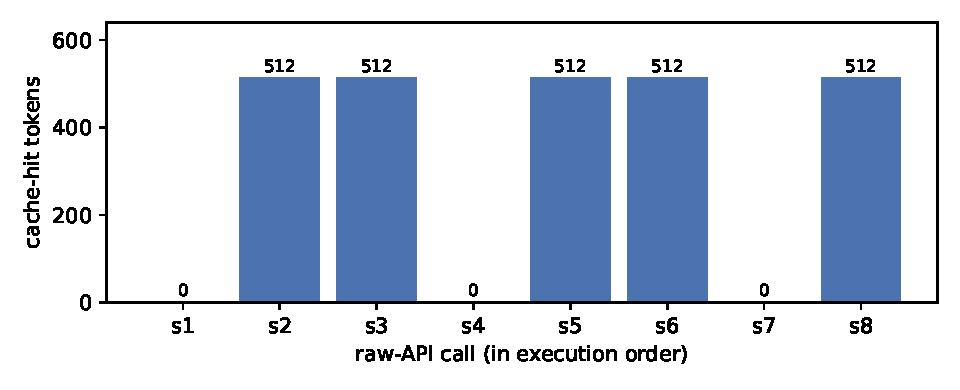
\includegraphics[width=0.86\textwidth]{figures/fig_hit.pdf}
\caption{通道 B 逐次调用的缓存命中 token 数。蓝色为同文档复用，红色为异文档对照，橙色为跨层级调用。}
\label{fig:hit}
\end{figure}

\textbf{持久性}：在上述序列完成约 35 分钟后，我们以同一文档再次发起调用（TTL 探针）：命中仍为 512 token，同批次的未见过文档命中为 0。这说明在本文的时间尺度内（分钟至半小时级），审计窗口是开放的；官方给出的清除语义为“数小时到数天”\cite{deepseekcache}，更长的窗口需要跨小时观测，留作后续工作。

\textbf{时延不构成替代信号}：flash 层命中调用的时延为 1.1--1.8 秒，flash 层未命中调用为 1.3--1.7 秒，二者不可分离；pro 层调用整体偏慢（3.4 秒）但与其条件无关。这与既有工作需要精心构造计时测量、并用分类器放大微弱差异的设定形成对照\cite{song2025earlybird}——在有账本可查的场景里，直接读计数即可。

\subsection{判定规则与文本基线}
\label{sec:results-rule}

对通道 B 的 7 个可判定调用（锚点之外的全部），判定规则~\eqref{eq:rule} 取得 7/7 的正确率：5 次同文档复用全部判为“复用”，异文档与跨层级调用均判为“未命中”。需要强调该规则的证据含义：对“同一服务模型内的上下文复用”，它是完美分离的；而跨层级条件下同一文档同样本命中为 0，意味着\textbf{“未命中”不能被解释为“来源不同”}（详见第~\ref{sec:discussion} 节）。

作为对照，我们计算生成文本之间的字符二元组 Jaccard 相似度：3 组可用文本对（因输出长度上限，部分回答被截断为空）中，同源对比 s2--s5 为 0.000，异源对比 s2--s4 也为 0.000，唯一非零值 s4--s5 为 0.051。也就是说，在这类“同底稿、不同问题”的复用场景中，\textbf{文本表面相似度几乎不携带信号}，而计量信号完全分离。

\section{讨论}
\label{sec:discussion}

\subsection{审计可用性取决于调用通道}
通道 A 的零命中不是平台能力缺失，而是调用链路设计的直接后果：agent 框架把\textbf{每次运行唯一的运行时路径}写入系统提示，使请求前缀在模型看到的第一个百 token 内即分叉，缓存匹配从结构上不可能发生。这对同类编排系统是可复现的结论——凡是把会话 ID、时间戳、工作目录等易变字段放入系统提示前部的链路，都会同时失去缓存的成本收益与计量取证信号。反过来，这给出两条可操作建议：（1）编排系统应把易变字段后置到稳定前缀之后，或放入用户消息尾部；（2）审计与合规场景应把“前缀稳定性”作为链路设计的显式约束。

\subsection{证据的不对称性}
规则~\eqref{eq:rule} 的证据意义是不对称的：命中是\textbf{强证据}（要出现非零命中，请求必须与既有缓存单元完全匹配，随机碰撞在实践中不可达）；未命中只是\textbf{弱否证}——它可能是真的未复用，也可能是复用发生但被三种情形掩盖：缓存被清除（官方为“数小时到数天”的尽力而为语义）、跨模型命名空间（表~\ref{tab:channelb} 中 s7：同文档、不同层级，命中为 0）、或前缀被运行时字段污染（通道 A）。跨层级不命中同时意味着一个实际后果：切换模型层级会同时损失成本复用一个取证通道，审计者必须限定“同一服务模型”比较。

\subsection{与标识制度的衔接}
计量取证在现行制度框架下有明确的落点：第九条的六个月日志留存义务使审计记录\textbf{天然可得}；第五、六条的元数据核验遇到的最大工程困难是标识在传播中丢失或被剥离，而计量证据不随内容传播——它留在服务提供者的账本里。因此，计量取证可作为隐式标识的\textbf{独立旁证通道}：用于核验“某批次内容是否源自同一底稿/同一素材”，或在标识与元数据相互矛盾时提供第三方视角。需要强调的是其边界：计量记录证明的是“上下文复用关系”，不是“内容由 AI 生成”，更不是“内容违法”；它服务于来源与传播链审计，而非生成判定。

\subsection{隐私与滥用风险}
同一信号对隐私是双刃的：能够识别“同一上下文被复用”，也意味着能够识别“某人反复使用同一段私有材料调用模型”。在平台侧，这类关联分析应被纳入最小必要与目的限定原则；在技术侧，可按租户隔离计量的可见粒度（本文实验未跨越账号边界，但机制上并不阻止同一账号内的高精度关联）。这一风险与缓存侧信道文献的关切同源，只是观测面从时序转移到了账面。

\subsection{局限}
（1）单一平台、单账号、单地域，结论的泛化需要多平台复现；（2）通道 A 的 17 次调用在同一部署内完成，未覆盖其它 agent 框架；（3）30 分钟空闲探针与 35 分钟 TTL 复测只能说明短时持久性，无法刻画官方语义中“数小时到数天”的清除边界；（4）样本规模小（通道 B 共 8 次），分离度结论是方向性的而非统计意义上的。

\section{结论}
\label{sec:conclusion}

本文把“AI 内容来源审计”从判断“是否生成”推进到判定“是否同源”，并提出与实证了一条此前未被系统考察的证据通道：服务端为计费而输出的上下文缓存计量。在真实平台上，该通道在裸 API 调用下可对“同一来源上下文”的实现复用给出完全分离的判定（512 vs 0 token，7/7 正确），并在分钟至半小时尺度上保持可用；而在 agent 编排链路上，同一平台、同一账号、同一材料的 17 次受控调用全部零命中——请求系统提示中嵌入的每次运行唯一路径在第 172 字符处破坏了前缀匹配。结论不是“某平台不可审计”，而是\textbf{审计可用性随调用链路设计而变}：它要求把“前缀稳定性”当作链路的一等约束，也要求审计方理解“未命中不等于不同源”的不对称语义。两个方向值得继续：跨小时与跨天的持久性边界，以及把计量证据与元数据标识做交叉核验的制度化接口。

\section*{数据与可复现性声明}
本文全部材料、调用脚本、逐次计量记录与分析脚本归档于项目仓库 \texttt{docs/\allowbreak papers/\allowbreak 2026-09-context-reuse-audit/}；分析脚本 \texttt{analysis/\allowbreak analyze.py} 可离线重放本文全部表格与图形。实验仅使用研究者原创材料与自有账号，未涉及任何第三方数据或跨账号观测。

% TODO(作者确认)：署名与单位（按新疆大学口径暂填），投稿前请核对姓名、邮箱与基金信息。

\bibliographystyle{unsrt}
\bibliography{refs}

\end{document}
